\documentclass{boi2014-lt}

\usepackage{enumitem}

\renewcommand{\DayNum}{2}
\renewcommand{\TaskCode}{postmen}
\renewcommand{\TaskName}{Senjorai paštininkai}

\begin{document}
    \begin{wrapfigure}[8]{r}{4cm}
        \vspace{-18pt}
		\includegraphics[width=4cm]{\TaskCode.jpeg}
	\end{wrapfigure}
    Dabar 2036-ieji metai ir Europa yra perpildyta garbaus amžiaus piliečiais.
    Tam, kad jie išsaugotų sveikatą, Europos daugumų ministerija (garbaus amžiaus
    piliečiai \emph{yra} dauguma!) siūlo įdarbinti juos popierinių laiškų,
    kurie vis dar yra siunčiama (dažniausiai būtent garbaus amžiaus piliečiams),
    išnešiotojais. Šis pasiūlymas bus realizuotas visoje Europoje, netgi
    nepriklausomose Norvegijos ir Šveicarijos valstijose.

    Ministerija sukūrė ``garbaus amžiaus piliečių sistemą'' padalindama visą
    Europą į pašto rajonus. Pašto rajoną -- tai gatvių tinklas, sudarytą iš
    gatvių ir sankryžų. Kiekviena gatve šiame tinkle galima eiti abejomis
    kryptimis. Kiekviename rajone paštininkais galima pasamdyti neribotą skaičių
    garbaus amžiaus piliečių. Kiekvieną rytą, kiekvienas paštininkas gauna krepšį
    su laiškais, kuriuos reikia pristatyti keliaujant maršrutu, dengiančiu dalį
    gatvių tinklo. Kiekvienas maršrutas turi būti tinkamas garbiam amžiui, t.~y.
    jis turi tenkinti šias sąlygas:
	%\todo{graph theory terminology here?}
    \begin{itemize}
        \item Prasidėti ir baigtis toje pačioje sankryžoje. (Hey, it’s a tour!)
        \item Nekirsti jokios sankryžos daugiau nei vieną kartą. (Nepainiokite
            garbaus amžiaus piliečių.)
        \item Neturėti bendrų gatvių su kitais maršrutais, t.~y. kiekvieną gatvę
            aptarnauja lygiai vienas paštininkas. (Garbaus amžiaus piliečiai
            neturėtų peštis tarpusavyje.)
    \end{itemize}

    Visi maršrutai kartu privalo pilnai padengti duotą gatvių tinklą: t.~y.
    kiekviena tinklo gatvė turi būti lygiai vieno maršruto dalimi.

    \Task
    Ministerija prašo jūsų sukurti programą, kuri duotam pašto rajono gatvių
    tinklui surastų garbiam amžiui tinkamų maršrutų aibę, kuri pilnai padengtų
    gatvių tinklą.

    \Input
    Įvestis apibūdina gatvių tinklą.
    
    Pirmoje eilutėje yra du sveikieji skaičiai $N$ ir $M$. $N$ -- sankryžų gatvių
    tinkle skaičius, $M$ -- gatvių tinkle skaičius. Sankryžos numeruojamos nuo
    $1$ iki $N$.

    Toliau kiekvienoje iš $M$ eilučių yra du sveikieji skaičiai $u$ ir $v$
    ($1 \le u, v \le N, u \neq v$), reiškiantys, kad šios gatvių sankryžos yra
    sujungtos gatve.

    Kiekvienai įvesčiai galioja:
    \begin{enumerate}
        \item Iš bet kurios sankryžos galima nukeliauti į bet kurią kitą.
        \item Sprendinys visada egzistuoja, t.~y. visada galima rasti garbiam
            amžiui tinkamų maršrutų aibę, kuri pilnai padengtų gatvių tinklą.
    \end{enumerate}

    \Output
    %\todo {fix the wording}
    Pirmoje eilutėje jūsų programa turi išvesti vieną sveikąjį skaičių $T$ --
    sudarytų maršrutų skaičių.

    Kitose $T$ eilučių įvardinkite $T$ maršrutų tokiu būdu: pirmasis skaičius
    eilutėje $C$ reikš, kiek skirtingų sankryžų paštininkas turi aplankyti šiame
    maršrute. Toliau išvardinti $C$ sveikųjų skaičių yra šių sankryžų numeriai.
    Sankryžos turi būti surūšiuotos taip, kad pirmasis išvestas numeris būtų
    maršruto pradžia ir pabaiga (ir jis būtų išvestas tik vieną kartą).

    Jeigu egzistuoja keletas sprendimų, jūsų programa gali išvesti bet kurų
    iš jų.

    \Example

    \example
    {
        10 15 \newline
        1 3 \newline
        5 1\newline
        2 3 \newline
        9 2\newline
        3 4 \newline
        6 3\newline
        4 5 \newline
        7 4\newline
        4 8 \newline
        5 7 \newline
        8 5\newline
        6 7 \newline
        7 8 \newline
        8 10 \newline
        10 9
    }
    {
        2 3 4 5 8 10 9 \newline
        4 7 8 \newline
        1 5 7 6 3
    }
    {
        Pateiktas paveiksliukas iliustruoja gatvių tinklą ir tris garbiam amžiui
        tinkamus maršrutus, kurie pilnai jį padengia.

        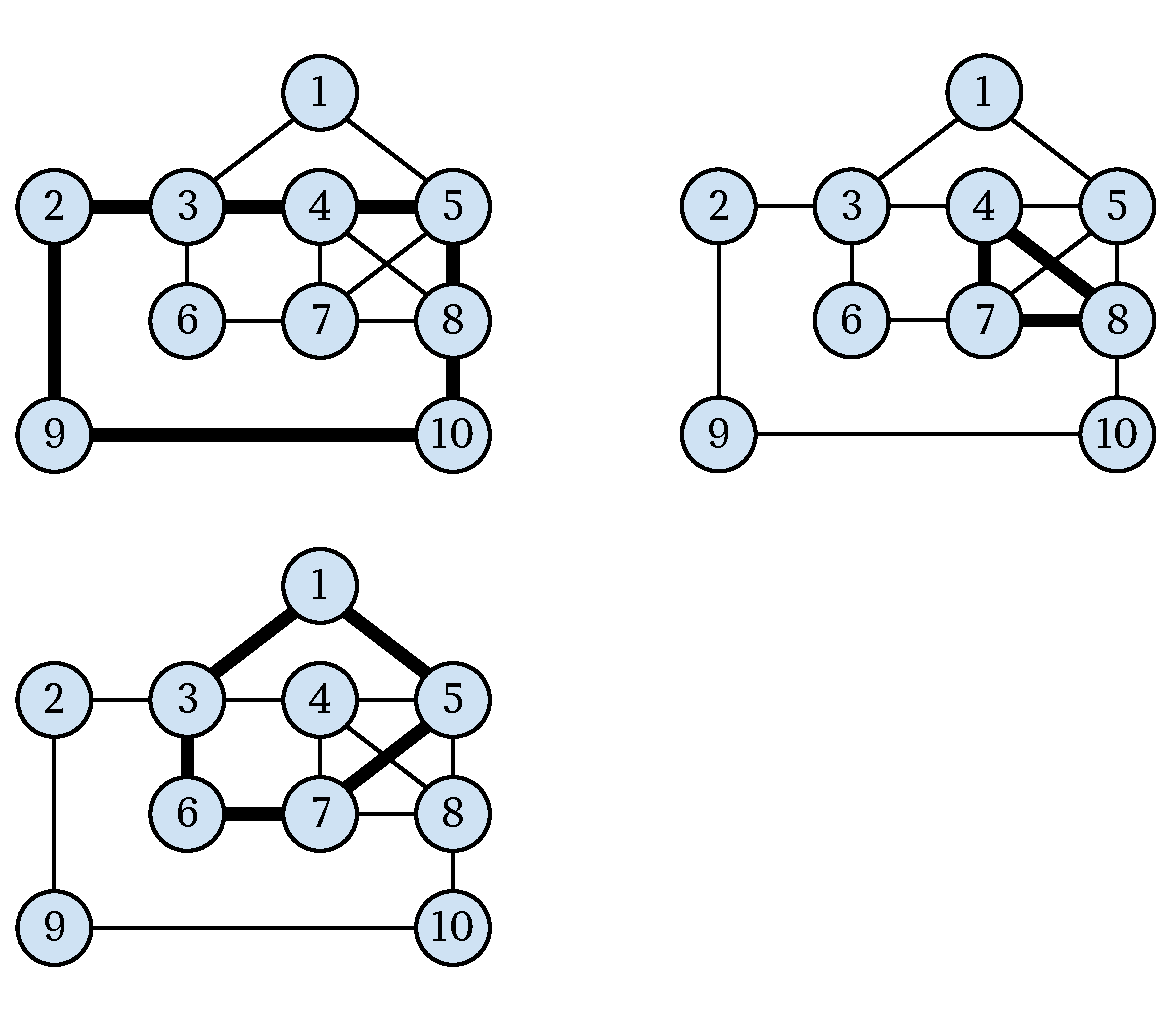
\includegraphics[width=7cm]{senior-example}

        Atkreipkite dėmesį, kad šiam pavyzdžiui egzistuoja keletas sprendimų,
        tame tarpe ir toks, kurį sudaro tik du maršrutai.
    }

    \Scoring

    \begin{description}
        \item[Dalinė užduotis nr. 1 (40 taškų):]
            $1 \le N \le 2\ 000$, $1 \le M \le 100\ 000$.
        \item[Dalinė užduotis nr. 2 (20 taškų):]
            $1 \le N \le 100\ 000$, $1 \le M \le 100\ 000$.
        \item[Dalinė užduotis nr. 3 (40 taškų):]
            $1 \le N \le 500\ 000$, $1 \le M \le 500\ 000$.
    \end{description}

    \Constraints

    \begin{description}
        \item[Laiko limitas:] 1 s.
        \item[Atminties limitas:] 256 MB.
    \end{description}

\end{document}
